\chapter{BPM in Industrie 4.0}
\section{RAMI 4.0}

\section{I4.0 component and Asset Administration Shell}

The \ac{AAS} contains and provides all relevant data and functions necessary to represent the physical asset in the information world. Figure \ref{fig:structureaas} shows the \ac{AAS} with its structure and characteristic features.

\begin{figure}[h]
\centering
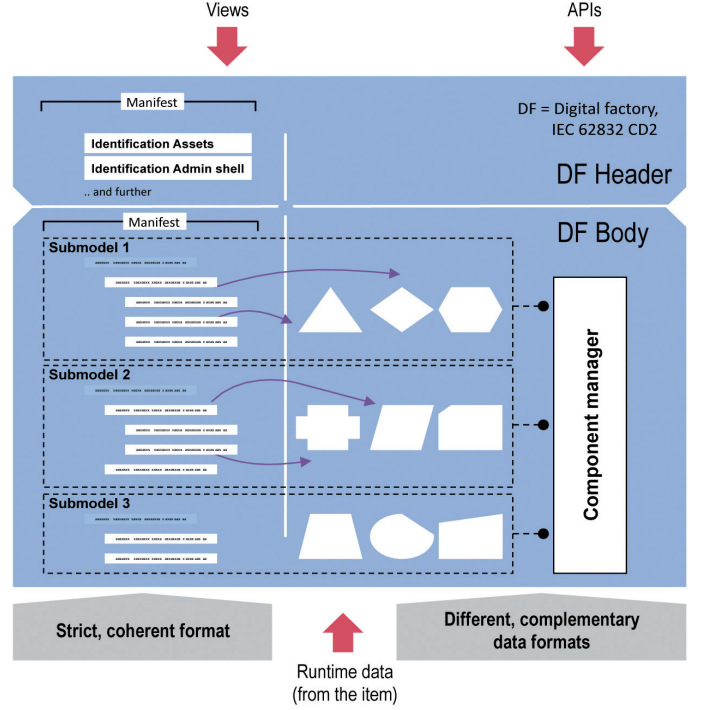
\includegraphics[scale=0.8]{content/pictures/structure_aas_zvei.png}
\caption{Structure of the Asset Administration Shell}
\source{\cite[p. 5]{Koschnick2016Beispiele4.0-Komponente-Basisteil}}
\label{fig:structureaas}
\end{figure}

The \ac{AAS} consists of two parts: The manifest and the component manager. The manifest contains metadata regarding the \ac{I4.0} component, such as a global unique identifier that can be used to identify the \ac{I4.0} component in the value chain. In addition, the metadata provides information whether the \ac{I4.0} component is of type or instance according to the life cycle \& value stream axis in \ac{RAMI4.0}. The component manager provides the uniform interface of the \ac{AAS}, through which the essential properties and functions of the asset can be realized. The component manager consists of several independent submodels, each of which describes exactly one property or function of the \ac{I4.0} component in a semantically uniform standard. By encapsulating the properties and functions in independent submodels, the integration of the \ac{I4.0} component in \ac{SOA} is made possible. This way, the component manager can be used to query exactly the property or call the function that is needed by other components in the system. Table \ref{tab:rotationspeedex} shows the exemplary structure of a submodel element for a feature rotation speed of a drilling machine.

\begin{table}[ht]
    \centering
    \begin{tabular}{|l||m{6cm}||l|}
    \hline
        \textbf{Property} & \textbf{Description} & \textbf{Value} \\ \hline
        Kind & Status of the asset in the lifecycle as defined by \ac{RAMI4.0} & INSTANCE  \\ \hline
        IdShort & Unique identification of the element itself & RotationSpeed  \\ \hline
        Category & Gives further meta-information regarding the type of the value & VARIABLE  \\ \hline
        Value & Observed or current value of the element & 4370   \\ \hline
        ValueType & Data type of the value & Integer\\ \hline
        SemanticId & Reference to the Semantic Dictionary either in or outside the \ac{AAS} & 18EBD56F6B43D895 \\ \hline
    \end{tabular}
    \caption{Example submodel for a property RotationSpeed}
    \label{tab:rotationspeedex}
\end{table}



\subsection{Interaction between I4.0 components}
As already outlined in \ref{chap:introduction} companies are moving towards \ac{SOA} to increase the flexibility of production to realize order-controlled production. This is necessary because in an \ac{I4.0}-compliant system no fixed allocation of production resources to the product being produced can be made in advance. Instead, production resources must be selected during runtime and configure themselves dynamically according to the given job \cite[p. 6]{Bock2016Weiterentwicklung4.0-Komponenten}. To realize this, the production resources under consideration for executing the needed production steps must interact with each other. The goal of the interaction is to determine which of the available resources can best meet the requirements for a given job in terms of cost, time and quality. Figure \ref{fig:relationshipppr} shows the relationship between product process and resource in an \ac{I4.0} system.

\begin{figure}[h]
\centering
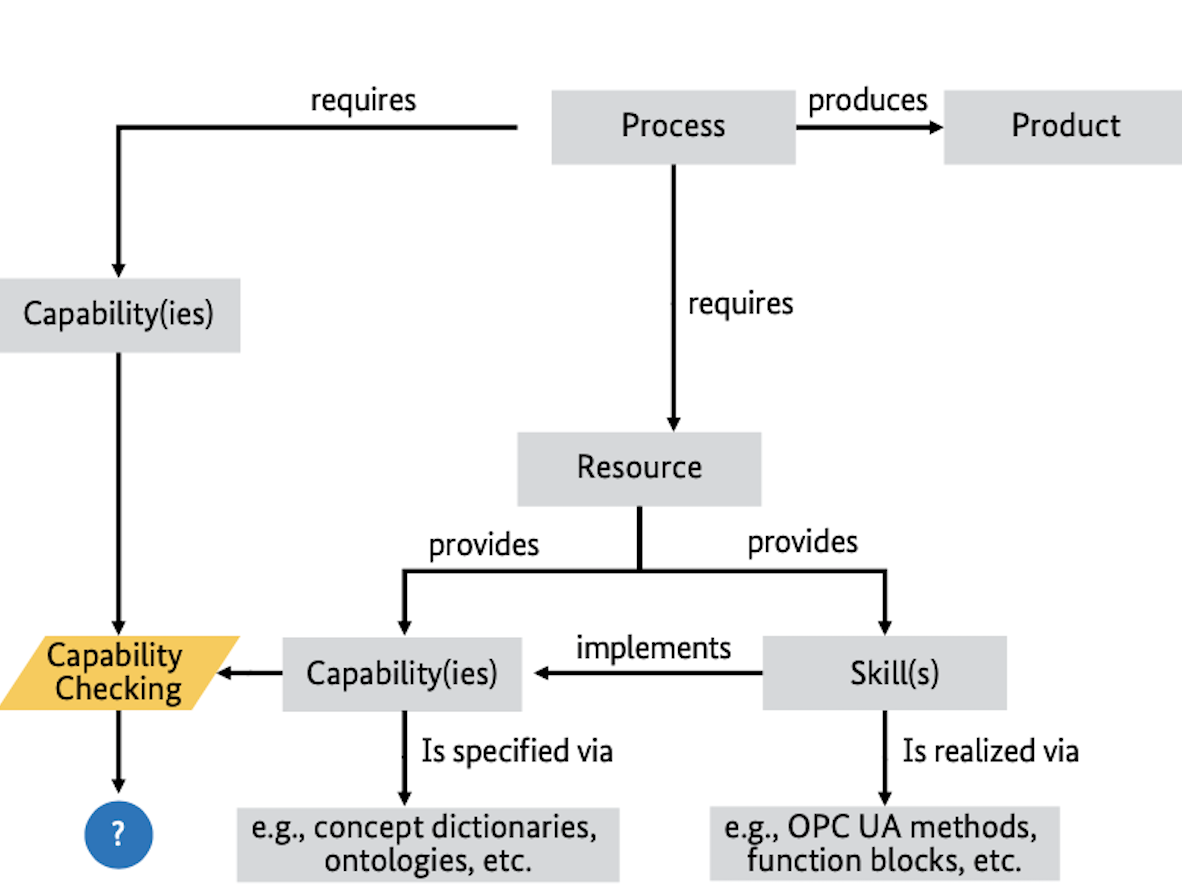
\includegraphics[scale=0.5]{content/pictures/relationship_product_process_resource.png}
\caption{Relationship between Product, Process and Resource in an I4.0 System}
\source{\cite[p. 5]{Bayha2020DescribingComponents}}
\label{fig:relationshipppr}
\end{figure}

The interaction to define the production process consists of two essential steps: capability and feasibility checking \cite[p. 6]{Bayha2020DescribingComponents}. To determine whether a resource within a value network is suitable in general for executing a given job, the capabilities and functionalities provided by the component are matched with the required resources for the process.

In order to be able to communicate both vertically and horizontally as part of an I4.0 system, a uniform set of rules must therefore be defined for communication so that messages can be exchanged between machines in a readable and interoperable manner. With the help of the \ac{I4.0} language, a set of grammar and rules are defined to make this possible. The Industrie 4.0 language defines three essential components for realization: vocabulary, message structure, and interaction protocols. These are described in the following.
